\documentclass[12pt]{article}


\usepackage{amssymb}
\usepackage{amsmath}
\usepackage{fullpage}
\usepackage{epsfig}
\usepackage{epstopdf}
\everymath{\displaystyle}



\begin{document}

\begin{center}
\underline{\LARGE{Length of a Plane Curve (Arc Length)}}
\end{center}

\bigskip

\noindent SUGGESTED REFERENCE MATERIAL:

\bigskip

\noindent As you work through the problems listed below, you should reference Chapter 6.4 of the recommended textbook (or the equivalent chapter in your alternative textbook/online resource) and your lecture notes.

\bigskip

\noindent EXPECTED SKILLS:

\begin{itemize}

\item Be able to find the arc length of a smooth curve in the plane described as a function of $x$ or as a function of $y$.

\end{itemize}

\noindent PRACTICE PROBLEMS:

\medskip

\noindent {\bf For problems 1-3, compute the exact arc length of the curve over the given interval.}

\begin{enumerate}

\item $y=4x^{\frac{3}{2}}-1$ from $x=\frac{1}{12}$ to $x=\frac{2}{9}$ 

\includegraphics[scale=0.5]{start.pdf}
{{$\frac{19}{54}$}}
\includegraphics[scale=0.5]{end.pdf}


\item $y = \frac{x^2}{2} - \frac{\ln(x)}{4}$ for $2 \leq x \leq 4$ 

\includegraphics[scale=0.5]{start.pdf}
{{$6+\frac{1}{4}\ln{2}$}}
\includegraphics[scale=0.5]{end.pdf}


\item $y=\frac{2}{3}(x^2-1)^{3/2}$ for $1\leq x \leq 3$ 

\includegraphics[scale=0.5]{start.pdf}
{{$\frac{46}{3}$}}
\includegraphics[scale=0.5]{end.pdf}


\item Consider the curve defined by $y = \sqrt{4-x^2}$ for $0 \leq x \leq 2$.

\begin{enumerate}

\item Compute the arc length on the interval $[0,t]$ for $0 \leq t <2$. (Your arc length will depend on $t$.)

\includegraphics[scale=0.5]{start.pdf}
{{$2\sin^{-1}{\left(\frac{t}{2}\right)}$}}
\includegraphics[scale=0.5]{end.pdf}


\item Use your answer from part (a) to compute the arc length on the interval $[0,2]$. (Hint: You will need to introduce a limit.)

\includegraphics[scale=0.5]{start.pdf}
{{$\pi$}}
\includegraphics[scale=0.5]{end.pdf}


\item Confirm your answer from part (b) by using geometry.

\includegraphics[scale=0.5]{start.pdf}
{{{1\linewidth}{On the interval $[0,2]$, the curve is $\frac{1}{4}$ of a circle with a radius of 2.  So, the length should be $\frac{1}{4}$  of the circumference; that is, $\text{Length} = \left.\frac{1}{4} \cdot 2 \pi r \right|_{r=2}= \frac{1}{4} \cdot 2 \pi (2) = \pi$.}}}
\includegraphics[scale=0.5]{end.pdf}


\end{enumerate}

\item Consider $F(x)=\int_1^x \sqrt{t^2-1} \,dt$.  Compute the arc length on $[1,3]$

\includegraphics[scale=0.5]{start.pdf}
{{4}}
\includegraphics[scale=0.5]{end.pdf}


\item Consider the curve defined by $f(x)=\ln{x}$ on $\left[1,e^3\right]$

\begin{enumerate}

\item Set up but do not evaluate an integral which represents the length of the curve by integrating with respect to $x$.

\includegraphics[scale=0.5]{start.pdf}
{{$L=\int_1^{e^3} \sqrt{1+\frac{1}{x^2}} \,dx$}}
\includegraphics[scale=0.5]{end.pdf}


\item Set up but do not evaluate an integral which represents the length of the curve by integrating with respect to $y$.

\includegraphics[scale=0.5]{start.pdf}
{{$L=\int_0^3 \sqrt{1+e^{2y}} \,dy$}}
\includegraphics[scale=0.5]{end.pdf}


\end{enumerate}

\item Consider the curve defined by $f(x)=\tan{x}$ on $\left[-\frac{\pi}{3},\frac{\pi}{4}\right]$

\begin{enumerate}

\item Set up but do not evaluate an integral which represents the length of the curve by integrating with respect to $x$.

\includegraphics[scale=0.5]{start.pdf}
{{$L=\int_{-\frac{\pi}{3}}^{\frac{\pi}{4}} \sqrt{1+\sec^4{x}} \,dx$}}
\includegraphics[scale=0.5]{end.pdf}


\item Set up but do not evaluate an integral which represents the length of the curve by integrating with respect to $y$.

\includegraphics[scale=0.5]{start.pdf}
{{$L=\int_{-\sqrt{3}}^{1} \sqrt{1+\frac{1}{(1+y^2)^2}} \,dy$}}
\includegraphics[scale=0.5]{end.pdf}


\end{enumerate}

\item Consider the curve defined by $y=\sin{x}$ for $0 \leq x \leq \pi$.

\begin{enumerate}

\item Set up but do not evaluate an integral which represents the length of the curve.

\includegraphics[scale=0.5]{start.pdf}
{{$\int_0^\pi \sqrt{1+\cos^2{x}} \,dx$}}
\includegraphics[scale=0.5]{end.pdf}


\item Estimate the value of your integral from part (a) by using a Midpoint Approximation with three rectangles of equal width.

\includegraphics[scale=0.5]{start.pdf}
{{{1\linewidth}{Below is the graph of $y=\sqrt{1+\cos^2{x}}$ on the interval $[0,\pi]$ along with three rectangles of equal width whose heights were determined by the function value at the midpoint of each resulting subinterval.\\
\begin{center}
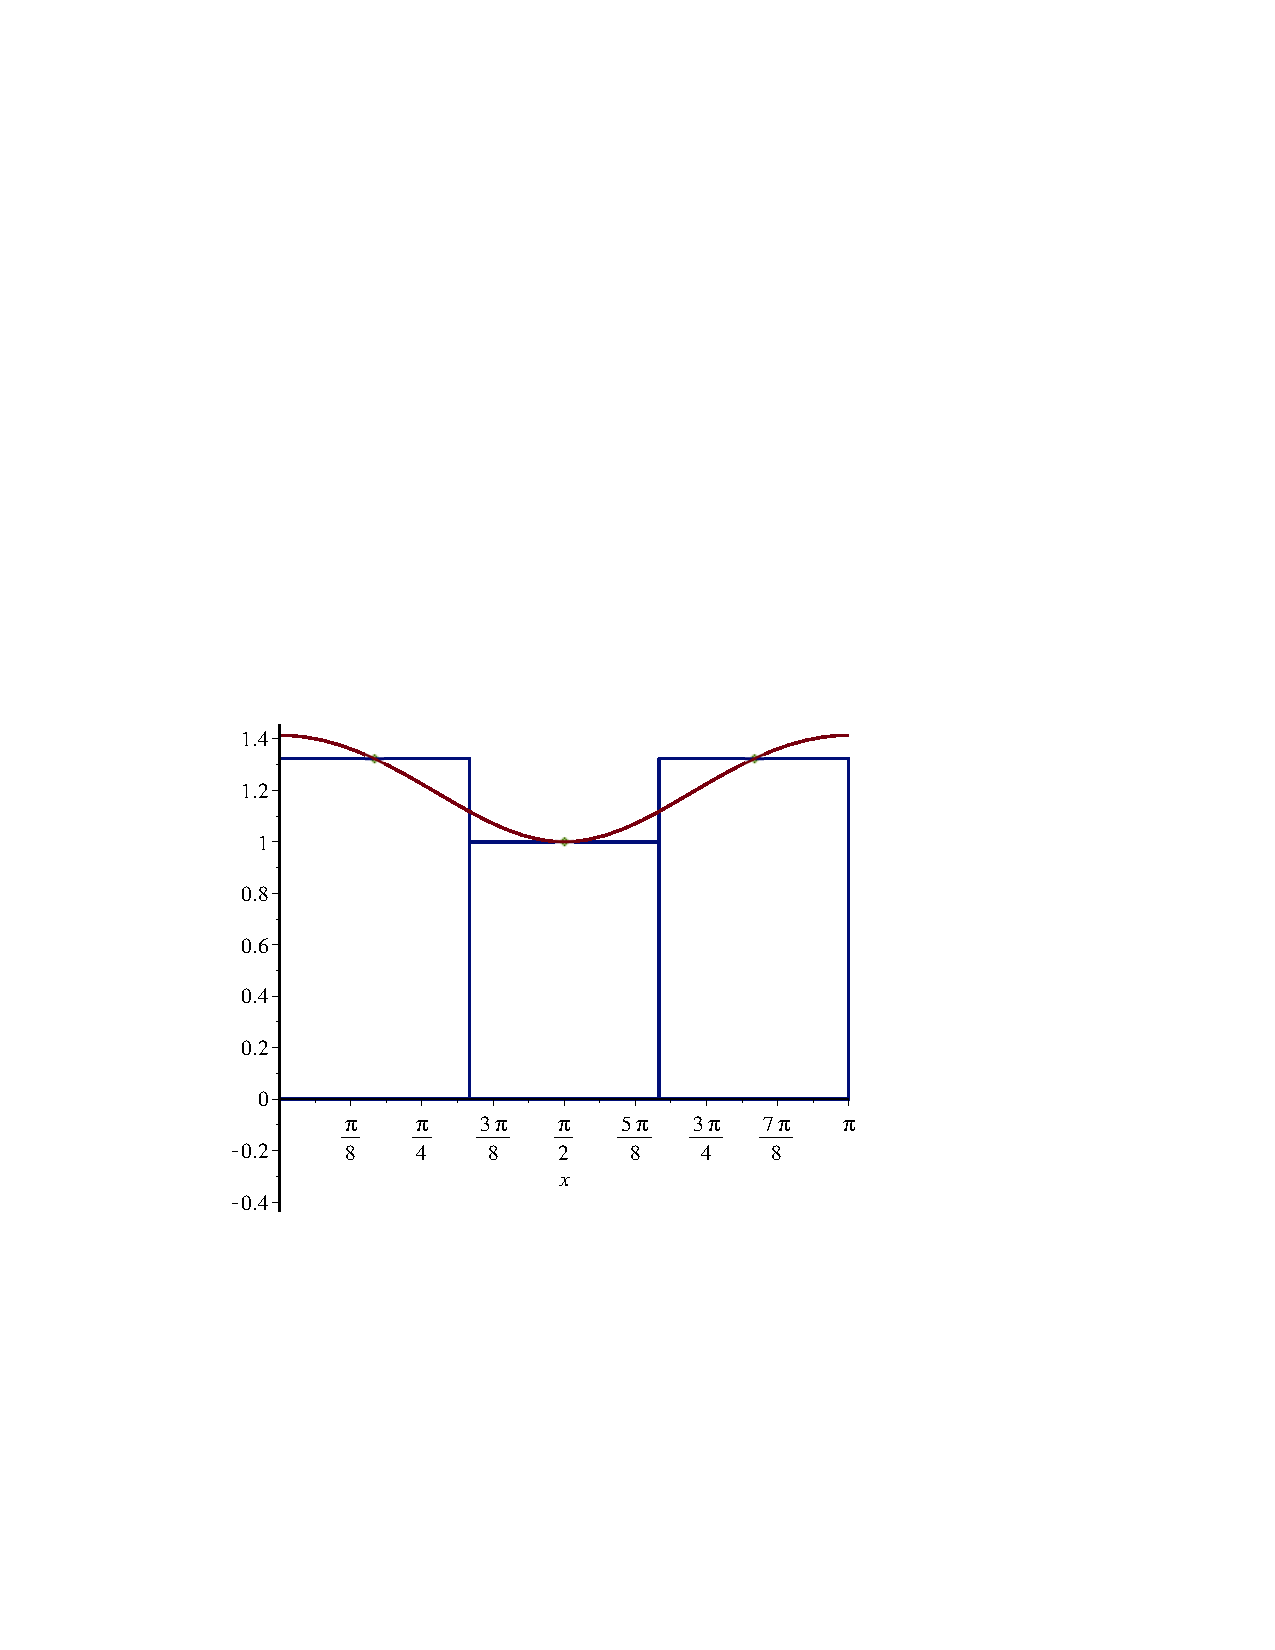
\includegraphics[scale=0.5]{Riemann_Sum.pdf}
\end{center}
Using these rectangles, $\int_0^\pi \sqrt{1+\cos^2{x}} \,dx \approx \frac{\pi}{3}\left(1+\sqrt{7}\right)$}}}
\includegraphics[scale=0.5]{end.pdf}


\end{enumerate}

\item Recall the definitions of Hyperbolic Sine \& Hyperbolic Cosine from Math 121:

\begin{center}
\begin{tabular}{ccc}
Hyperbolic Sine & & Hyperbolic Cosine\\
& & \\
$\sinh{x}=\frac{e^x-e^{-x}}{2}$ & \hspace{1 cm} & $\cosh{x}=\frac{e^x+e^{-x}}{2}$
\end{tabular}
\end{center}

\smallskip

The sketches of $y=\cosh{x}$ and $y=\sinh{x}$ are shown below.  The dashed curves are called ``Curvilinear Asymptotes," which describe the end behavior of the functions.
\begin{center}
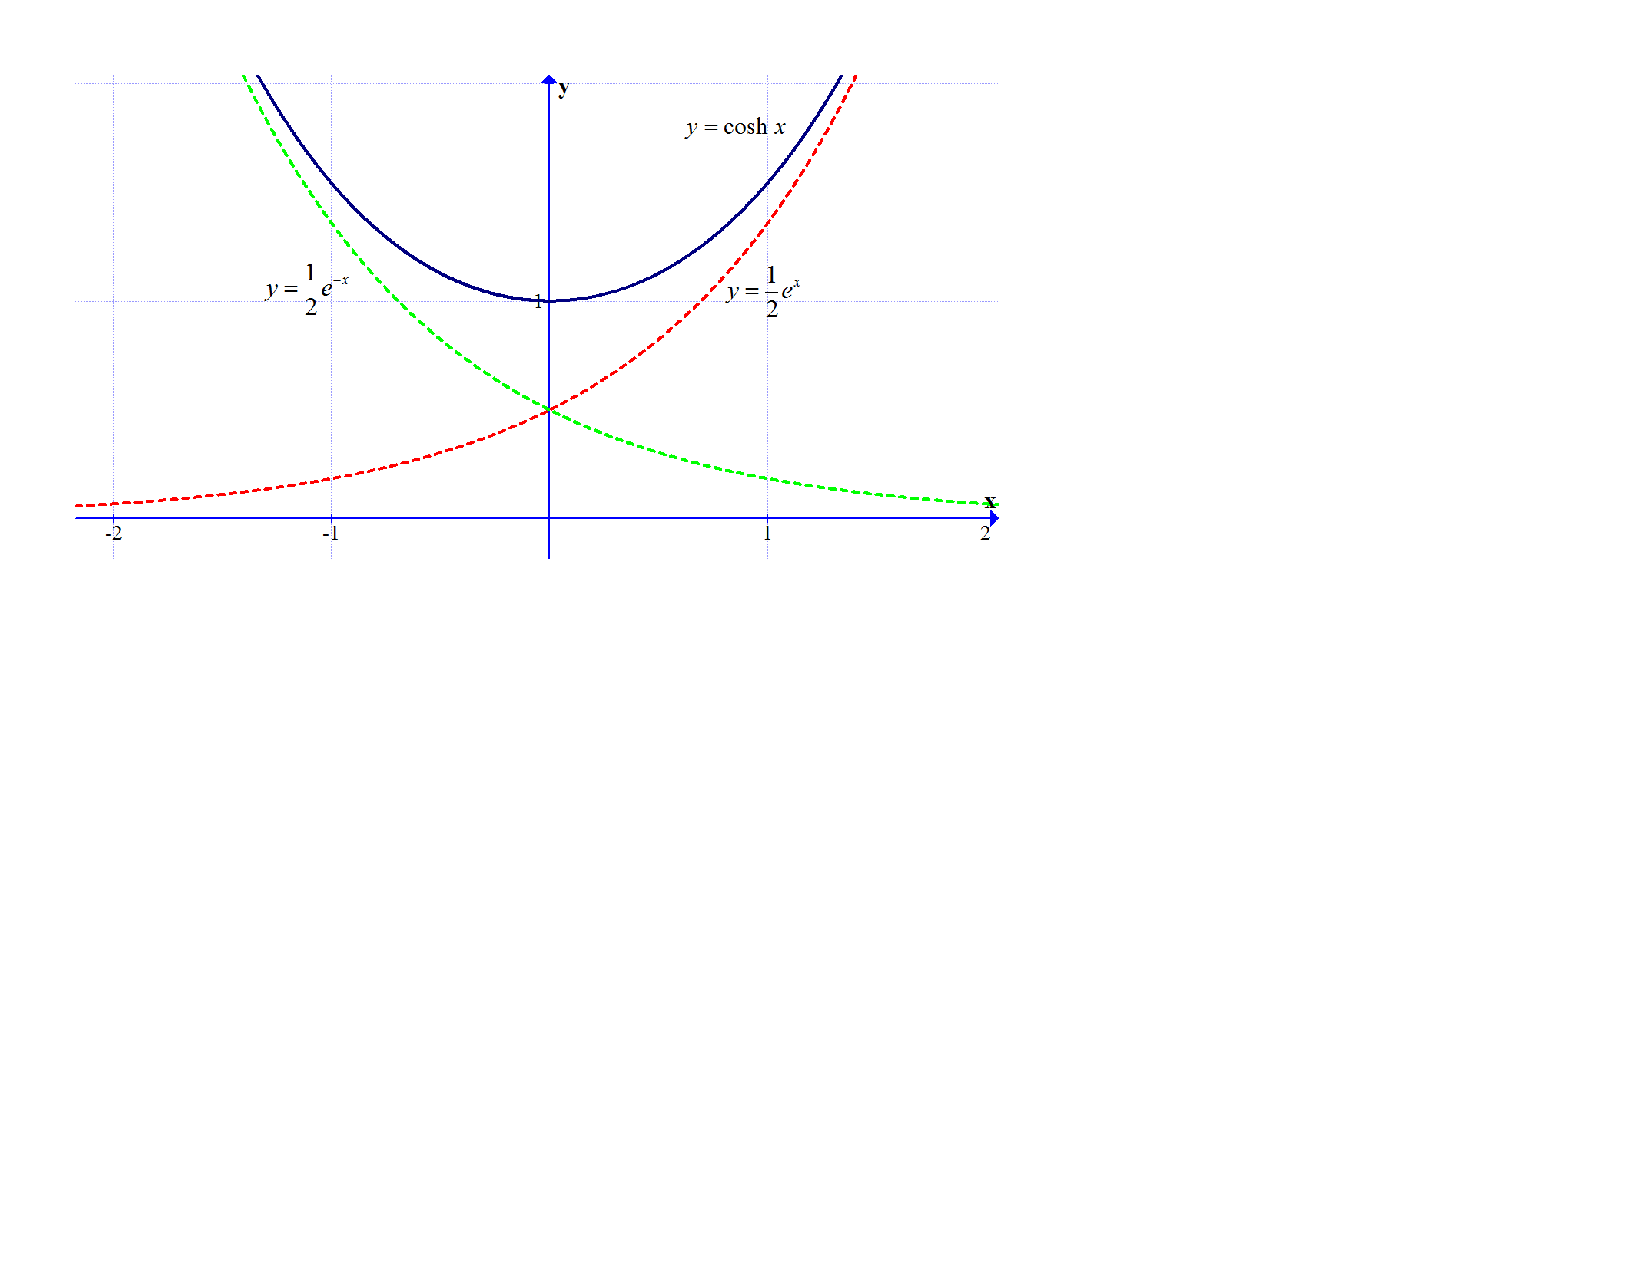
\includegraphics[scale=0.6]{cosh.pdf}\\
\vspace{0.5 cm}
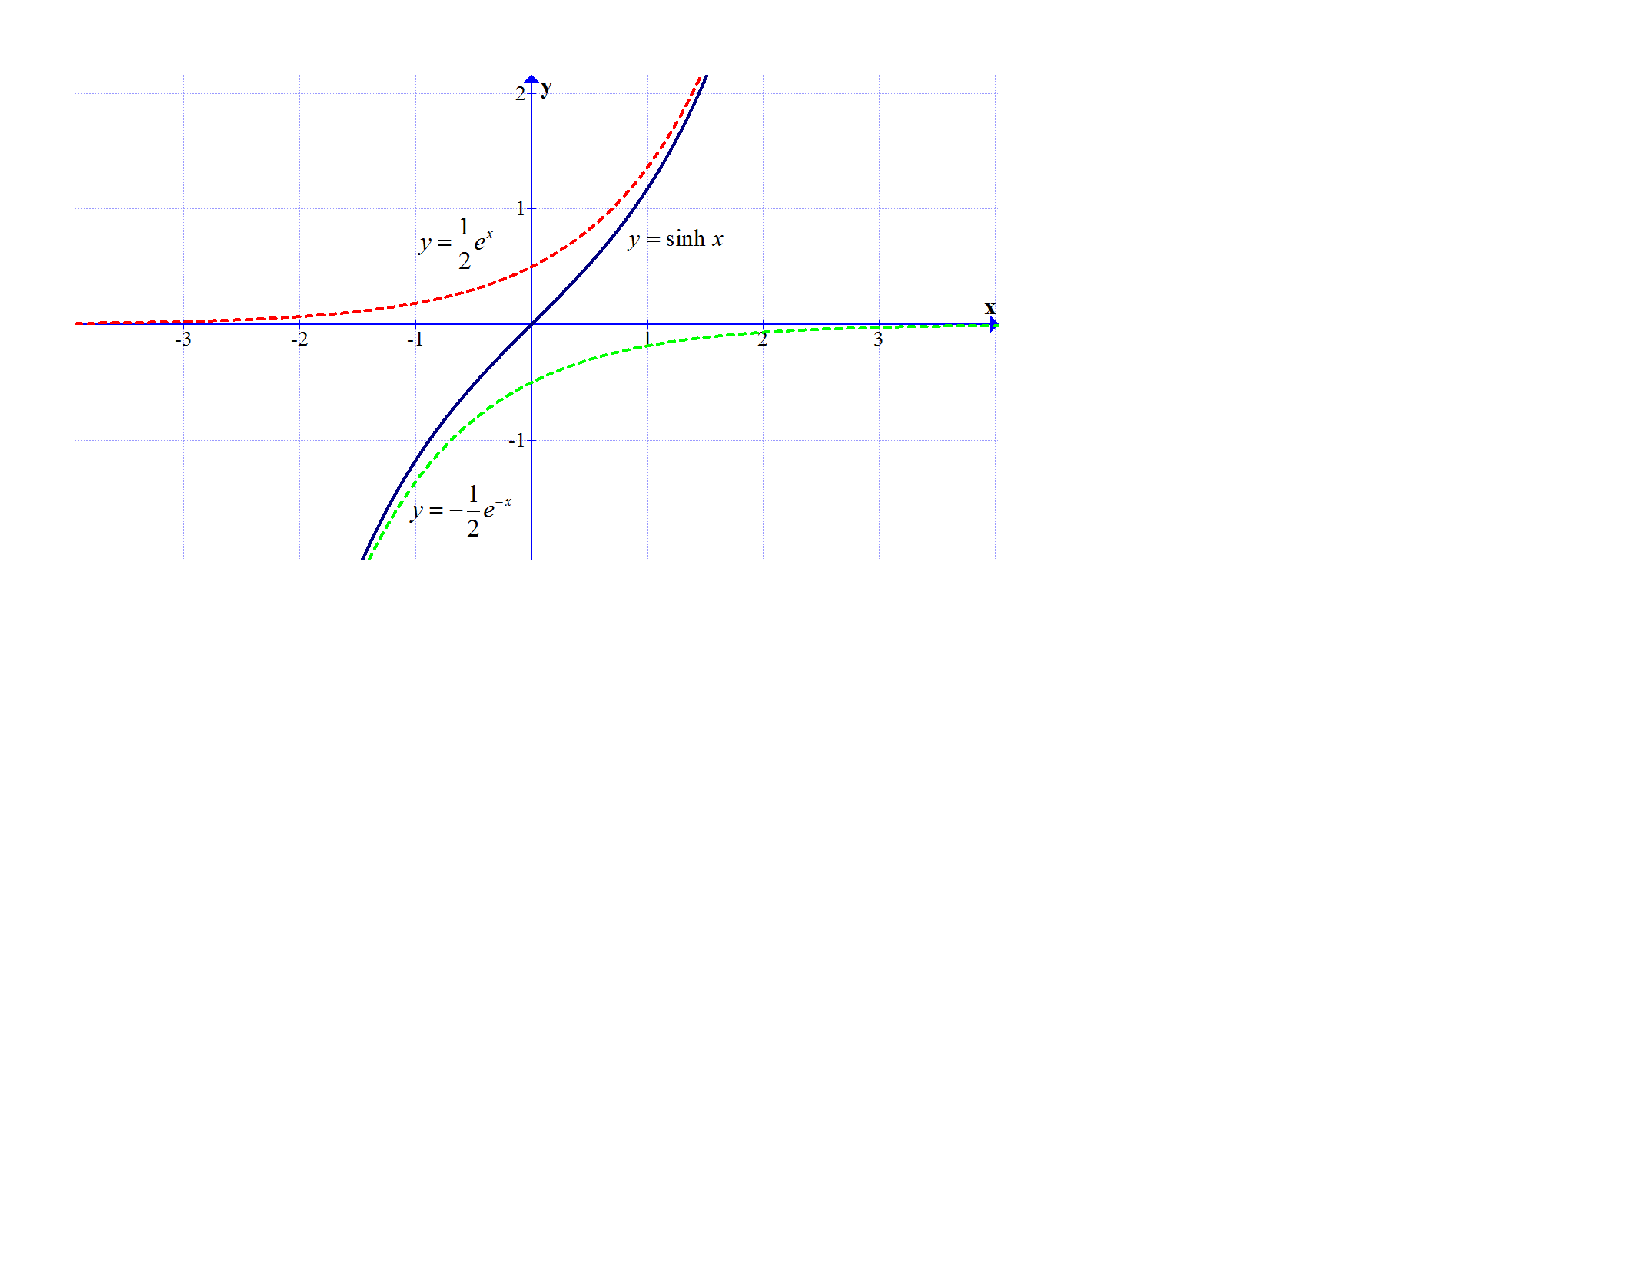
\includegraphics[scale=0.6]{sinh.pdf}
\end{center}

\begin{enumerate}

\item Show that $\cosh^2{x}-\sinh^2{x}=1$

\includegraphics[scale=0.5]{start.pdf}
{{{1\linewidth}{
\begin{align*}
\cosh^2{x}-\sinh^{2}{x} & = (\cosh{x}+\sinh{x})(\cosh{x}-\sinh{x})\\
&=\left(\frac{e^x+e^{-x}}{2}+\frac{e^x-e^{-x}}{2}\right)\left(\frac{e^x+e^{-x}}{2}-\frac{e^x-e^{-x}}{2}\right)\\
&=(e^x)(e^{-x})\\
&=1
\end{align*}
}}}
\includegraphics[scale=0.5]{end.pdf}


\item Verify that $f(x)=\sinh{x}$ is an odd function. ({\bf Hint:} Recall an odd function satisfies the identity $f(-x)=-f(x)$.)

\includegraphics[scale=0.5]{start.pdf}
{{{1\linewidth}{To verify that a function is off, we check that $f(-x)=-f(x)$. We compute by appealing to the definition of $\sinh{x}$ from above.
\begin{align*}
\sinh{(-x)}&=\frac{e^{-x}-e^{-(-x)}}{2}\\
&=\frac{e^{-x}-e^{x}}{2}\\
&=-\left(\frac{e^{x}-e^{-x}}{2}\right)\\
&=-\sinh{x}
\end{align*}
Thus, $f(x)=\sinh{x}$ is odd.}}}
\includegraphics[scale=0.5]{end.pdf}


\item Show that $\frac{d}{dx}(\sinh{x})=\cosh{x}$ and deduce that $\int \cosh{x}\,dx=\sinh{x}+C$.

\includegraphics[scale=0.5]{start.pdf}
{{{1\linewidth}{
\begin{align*}
\frac{d}{dx}(\sinh{x}) &= \frac{d}{dx}\left(\frac{e^x-e^{-x}}{2}\right)\\
&=\frac{d}{dx}\left(\frac{1}{2}e^x-\frac{1}{2}e^{-x}\right)\\
&=\frac{1}{2}e^x+\frac{1}{2}e^{-x}\\
&=\frac{e^x+e^{-x}}{2}\\
&=\cosh{x}
\end{align*}
Thus, as a result, $\int \cosh{x}\,dx=\sinh{x}+C$.  (We could have also verified this integration formula by integrating the given definition of $\cosh{x}$.)
}}}
\includegraphics[scale=0.5]{end.pdf}


\item Show that $\frac{d}{dx}(\cosh{x})=\sinh{x}$ and deduce that $\int \sinh{x}\,dx=\cosh{x}+C$.

\includegraphics[scale=0.5]{start.pdf}
{{{1\linewidth}{
\begin{align*}
\frac{d}{dx}(\cosh{x}) &= \frac{d}{dx}\left(\frac{e^x+e^{-x}}{2}\right)\\
&=\frac{d}{dx}\left(\frac{1}{2}e^x+\frac{1}{2}e^{-x}\right)\\
&=\frac{1}{2}e^x-\frac{1}{2}e^{-x}\\
&=\frac{e^x-e^{-x}}{2}\\
&=\sinh{x}
\end{align*}
Thus, as a result, $\int \sinh{x}\,dx=\cosh{x}+C$.  (We could have also verified this integration formula by integrating the given definition of $\sinh{x}$.)
}}}
\includegraphics[scale=0.5]{end.pdf}


\item A telephone wire which is supported only by two telephone poles will sag under its own weight and form the shape of a {\bf catenary} as shown below.

\begin{center}
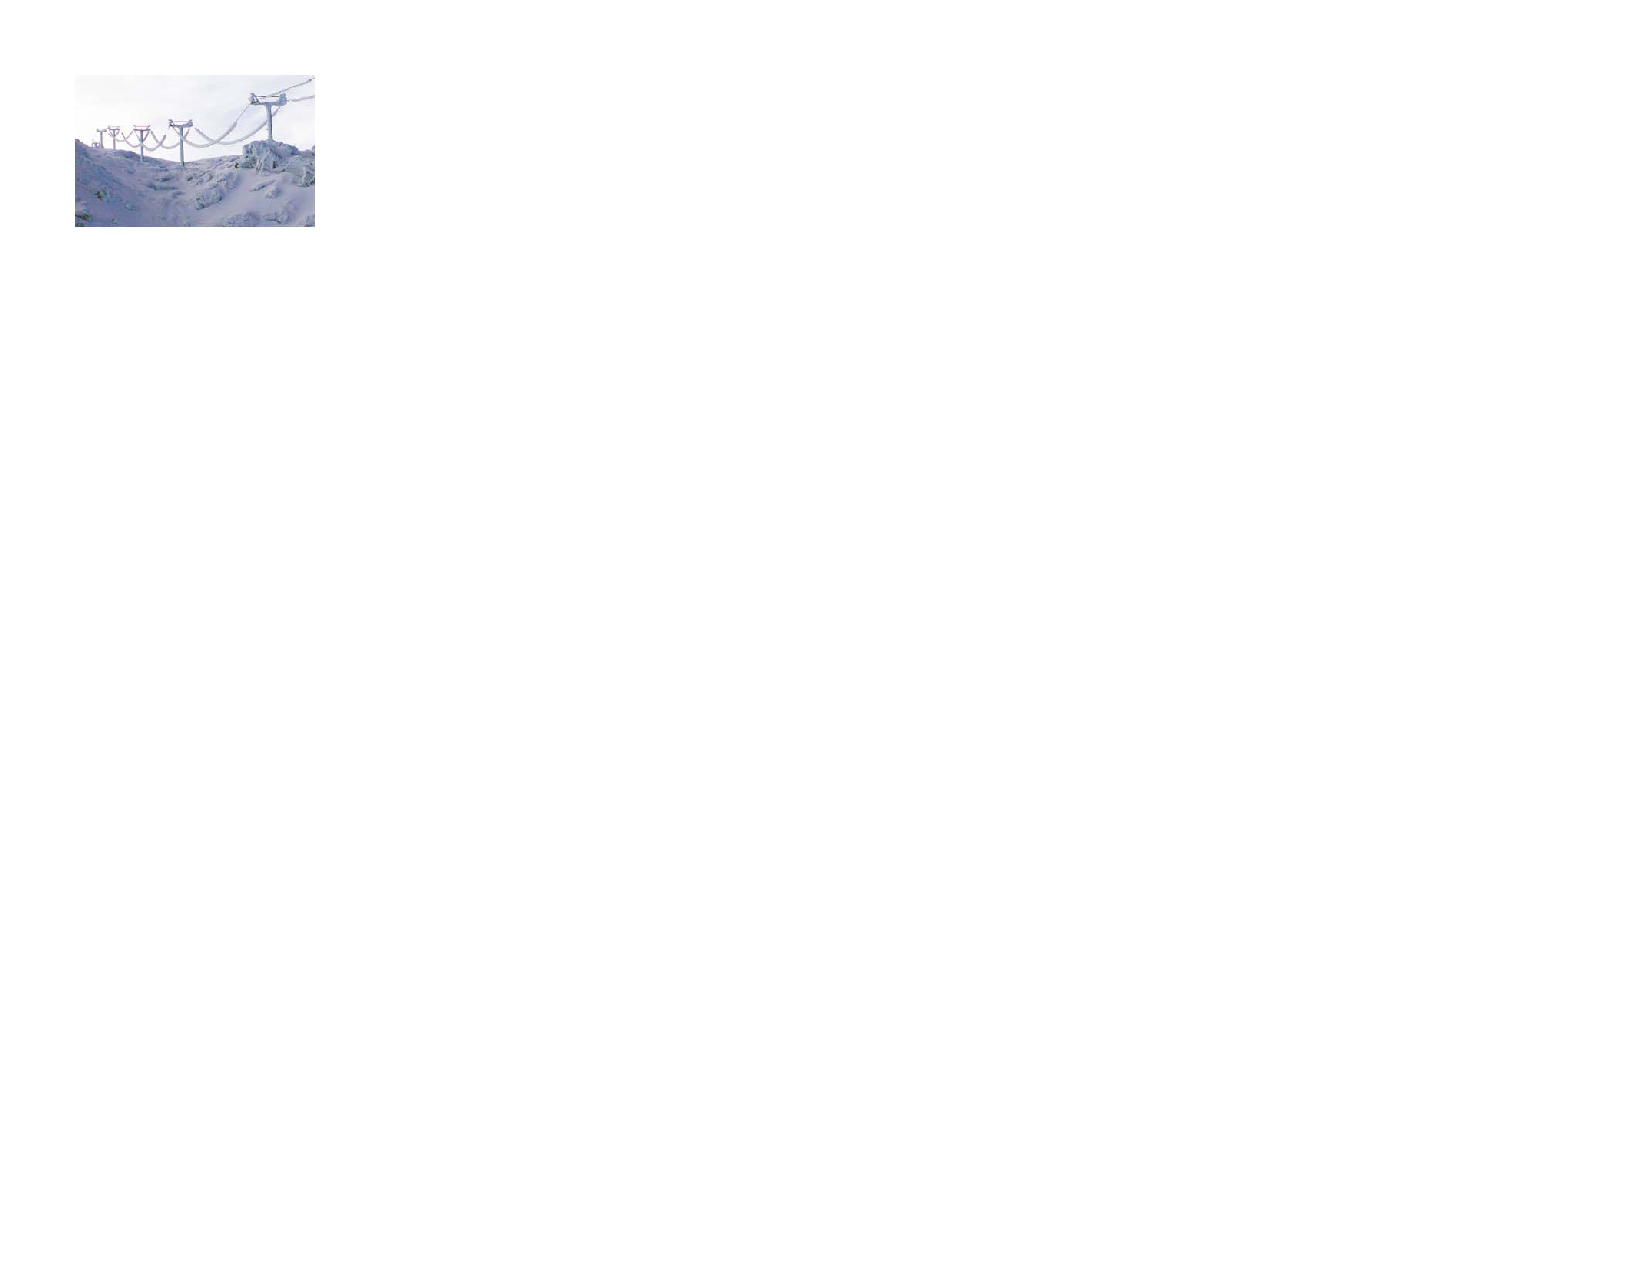
\includegraphics[scale=1]{catenary.pdf}
\end{center}

Consider a telephone wire that is supported by two poles (one at $x=b$ and the other at $x=-b$), as in the diagram below.

\begin{center}
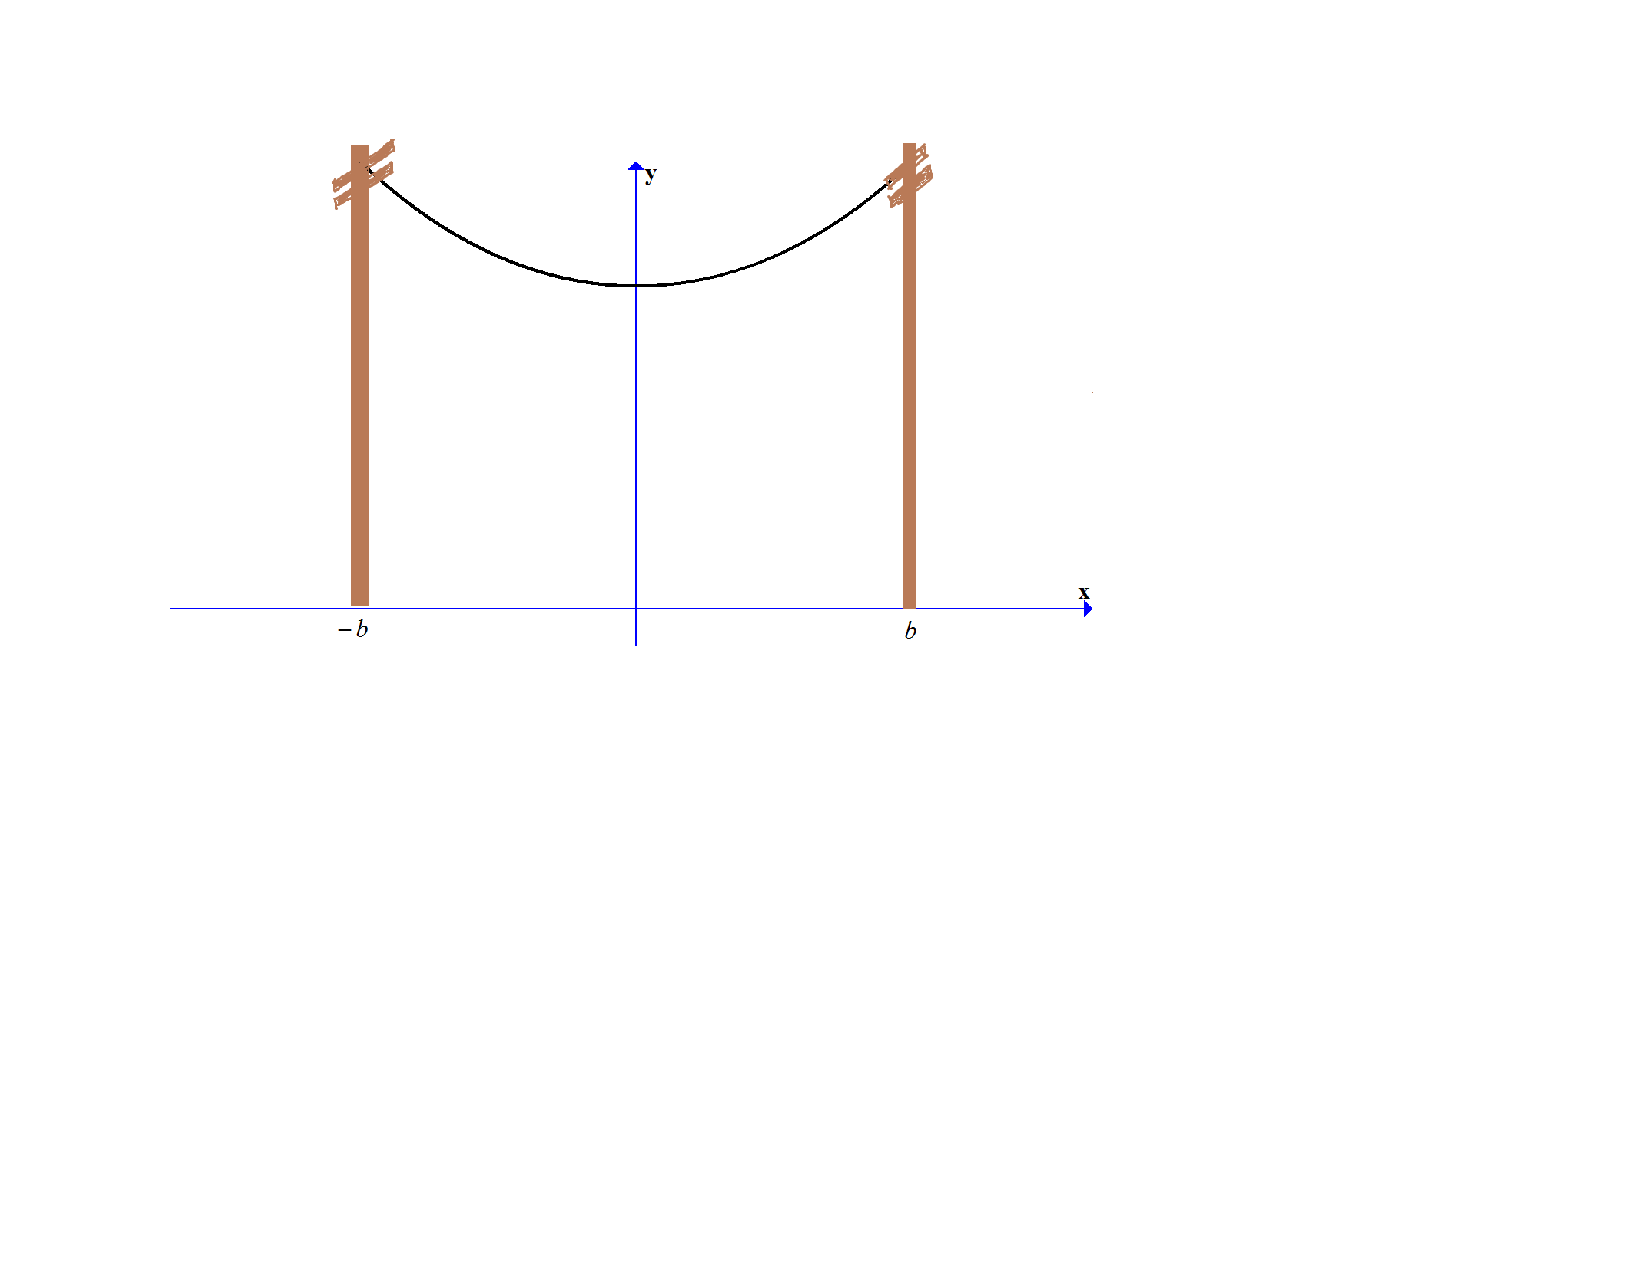
\includegraphics[scale=0.6]{catenary2.pdf}
\end{center}

The shape of the sagging wire can be modeled by $y=a\cosh{\left(\frac{x}{a}\right)}$, where $a>0$ and $-b \leq x \leq b$.  What is the length of the wire?

\includegraphics[scale=0.5]{start.pdf}
{{$A=2a\sinh{\left(\frac{b}{a}\right)}$}}
\includegraphics[scale=0.5]{end.pdf}


\end{enumerate}

\end{enumerate}

\end{document}